\documentclass[a4paper, 12pt,oneside]{article} 
%\documentclass[a4paper, 12pt,oneside,draft]{article} 

\usepackage{preamble}
\usepackage{bm}

%--------------------- ACTUAL FILE ---------------------- %
\begin{document} 
	\begin{center}
	    \Large
	    \textbf{RL mini-project : Mountain Car environment}
	        
	    \vspace{0.4cm}
	    \large
	    Authors : Rayan Harfouche \& Tara\footnote[1]{My administrative name is Tobia, so you will find me under that name in EPFL related databases.} Fjellman \\
	    \small{Spring 2024}
	\end{center}

    \section{Introduction}
        In this report we analyze and compare algorithms on the continuous Mountain Car RL environment. We consider versions of a model model-free algorithm (DQN) and a model-based one (Dyna). 
    \section{Random agent}
    \begin{wrapfigure}[14]{r}{0.45\textwidth}
        \centering
        \vspace{-3em}
        \includegraphics[width=0.45\textwidth]{random/n_eps=1000/figs/duration}
        \caption{Episode duration of random agent during training.}
        \label{fig:random-neps=1000}
    \end{wrapfigure}
    We start by running an agent that selects its actions at random. To analyze its performance, we inspect the duration of the episodes. Indeed, if the agent solves the task, the duration of the episodes should be lower than 200\footnote[2]{... of course except if it solves the task in exactly 200 steps.} (as this is the truncation time).
    Running the agent for 1000 episodes, we obtain \ref{fig:random-neps=1000}. Looking at it, it is clear that the agent does not succeed at the task. Actually, the agent just oscillates around the minimum. The reason for which the reward and loss are 0 for the first 40 episodes is that they are only computed once the buffer has been filled.  
    \section{DQN}
        \subsection{Vanilla version}
        \begin{figure}[h!]
            \centering
            \vspace{0em}
                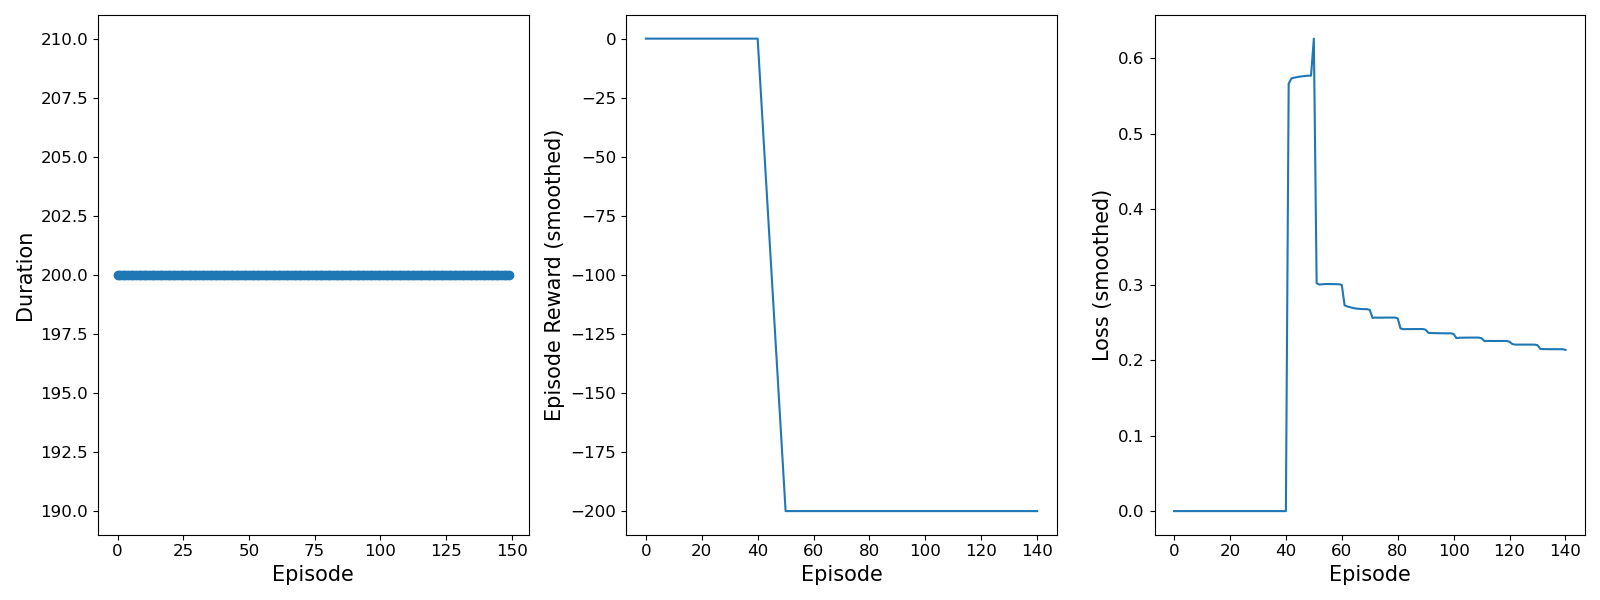
\includegraphics[width=.9\textwidth]{dqn_vanilla/up-tau=3/figs/full_results}
                \caption{Results associated to the training of a vanilla DQN agent.}
                \label{fig:dqn-vanilla-neps=1000}
        \end{figure}
        We now turn to the DQN agent. 
        Running 1000 episodes and computing : the duration of the episodes along with the episode-cumulated reward and loss, we get \ref{fig:dqn-vanilla-neps=1000}. Looking at it we see that the behavior is similar to that of the random agent, i.e. the agent does not learn the task. There are only a few sparse successes. This is due to the sparsity of the reward. Indeed, without reward, the agent cannot inform its policy updates. 
        \subsection{Auxiliary reward}
        In this section we consider DQN agents auxiliary rewards, with the goal of countering the reward sparsity. 
        \subsubsection{Heuristic reward}
        \subsubsection{Choosing the function}
        \begin{wrapfigure}{r}{0.45\textwidth}
            \centering
            \vspace{-6em}
            \includegraphics[width=0.45\textwidth]{dqn_heuristic/up-tau=3_d=2_frac=0.7-long/figs/loss}
            \caption{Evolution of episode training loss for a heuristic reward agent. The reward factor is set to 0.7 and smoothing with a window of width 10 is applied.}
            \label{fig:dqn-heuristic-frac=0.7-loss}
        \end{wrapfigure}
        As we want this function to reward the agent when it makes an effort to reach the top of the hill, it makes sense for it to be monotonous in the height $h(x)$ of the car. The (normalized) height can be deduced from the position as $h(x) = \frac{1}{2}\{1-\cos[(x-x_0)\pi/(x_r-x_0)]\}$ where $x_0$ and $x_r$ respectively are the average-starting and ending positions. 
        A simple and versatile reward function is therefore $f(x) = Ah(x)^n$
        for $A\ge 0$ some constant we call reward-factor and a given exponent $n\in\mathbb N^\star$ (which we take as $n=2$ from now on). 
        To check that this agent is learning we look at the evolution of the loss in \ref{fig:dqn-heuristic-frac=0.7-loss}, the duration in \ref{fig:dqn-heuristic-frac=0.7-duration} and the collected reward in \ref{fig:dqn-heuristic-frac=0.7-reward}. Looking first at \ref{fig:dqn-heuristic-frac=0.7-duration}, we see that the agent learns to  solve the task in less than 500 episodes. 
        \begin{figure}[h!]
            \centering
            \vspace{0em}
            \includegraphics[width=.65\textwidth]{dqn_heuristic/up-tau=3_d=2_frac=0.7-long/figs/duration}
            \caption{Evolution of episode duration and cumulative number of successes for a heuristic reward agent. The reward factor is set to 0.7.}
            \label{fig:dqn-heuristic-frac=0.7-duration}
        \end{figure}

        \begin{wrapfigure}[13]{r}{0.65\textwidth}
            \centering
            \vspace{-2em}
            \includegraphics[width=.65\textwidth]{dqn_heuristic/up-tau=3_d=2_frac=0.7-long/figs/reward}
            \caption{Evolution of cumulative reward and cumulative reward cumulated over the episodes for a heuristic reward agent. The reward factor is set to 0.7 and the cumulative reward is smoothed with a window of width 10.}
            \label{fig:dqn-heuristic-frac=0.7-reward}
        \end{wrapfigure}
        Now turning to \ref{fig:dqn-heuristic-frac=0.7-reward}, we see it matches our expectations. Indeed, at the start (for $N_{eps}\le 200$) the auxiliary reward increases, promoting exploration of higher states. Then, the environment reward increases as the agent has learned to solve the task. 
        As for the loss, we see that it is increasing, which might come to a surprise (as in ML we are used to seeing training losses decrease). In this case however, the loss is just an indicator of how well the agent is learning the Q function. The observed increase therefore is attributed to the fact that the learning of this function gets harder as its domain increases (training on new states, we increase the difficulty of matching the target). We expect this loss to start decreasing once the learned policy will be closer to its equilibrium. 
        \subsubsection{Auxiliary reward scaling}
        \begin{wrapfigure}{r}{0.65\textwidth}
            \centering
            \vspace{-1em}
            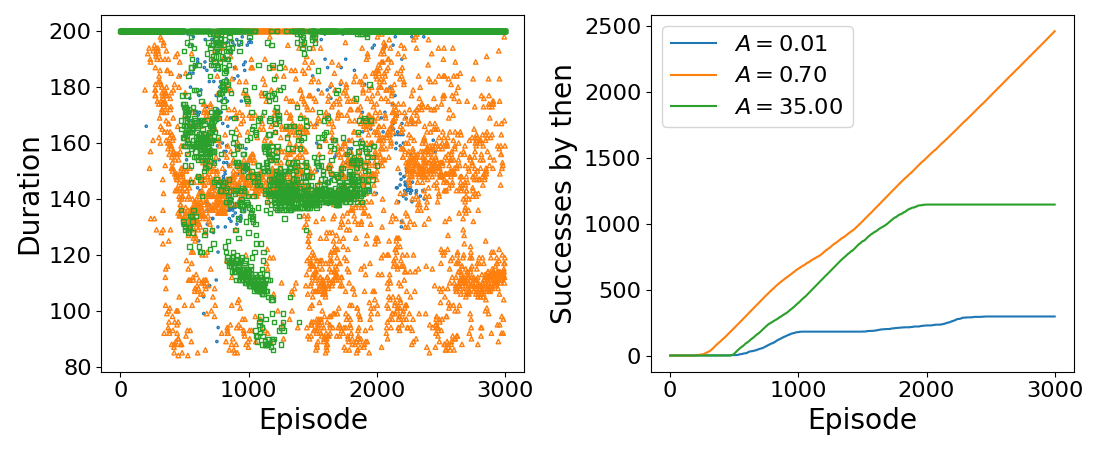
\includegraphics[width=.67\textwidth]{dqn_heuristic/heuristic_comparison}
            \caption{Evolution of episode duration and cumulative number of successes for heuristic reward agents. The different colors correspond to different values of the reward factor.}
            \label{fig:dqn-heuristic-comparison}
        \end{wrapfigure}
        For the auxiliary reward to be useful we want it to be : (a) sufficiently large for the agent to differ from the vanilla one; and (b) small enough not to dominate the environment reward (otherwise the agent will learn to optimize it instead of the environment reward). The exact optimal value is not easy to express analytically, but we expect it to be around the order of 1. This provides us with a crude guess, which we can refine by testing different values.
        We now analyze the effect of the reward factor on the performance, by considering multiple values for it. The corresponding results are shown in \ref{fig:dqn-heuristic-comparison}. We indeed observe the described trends. For $A=0.01$ the duration plot looks similar to what happens for the vanilla DQN : the incentive to explore higher states is too low. For $A=35$ we see that the agent first learns the task, but then realizes that doing so (and thereby shortening episodes) conflicts with the harvesting of the auxiliary reward, and so unlearns the task.
        \section{RND reward}
        \begin{wrapfigure}[14]{r}{0.45\textwidth}
            \centering
            \vspace{-2em}
            \includegraphics[width=0.45\textwidth]{dqn_rnd/up-tau=1_r-fact=10.0/figs/loss}
            \caption{Evolution of episode training loss for an RND reward agent. The reward factor is set to 10 and the loss is smoothed with a window of width 10.}
            \label{fig:dqn-rnd-r-fact=10-loss}
        \end{wrapfigure}
        In this section we consider the results of the RND auxiliary reward agent.
        First we can proceed as for the previous agent by plotting the evolution of the loss in \ref{fig:dqn-rnd-r-fact=10-loss}, the duration in \ref{fig:dqn-rnd-r-fact=10-duration} and the collected reward in \ref{fig:dqn-rnd-r-fact=10-reward}. Looking first at \ref{fig:dqn-rnd-r-fact=10-duration}, we see that the agent learns to  solve the task in less than 500 episodes. 
        \subsection{Normalization} 
        As recommended by the hint, we standardize the input and output of the RND network. The input standardization is done since we want the output to vary as a function of how different the observed state is compared to the previously visited ones. Indeed, subtracting the typical state (i.e. the mean one) provides a good idea of how different the new input state is.
        The normalizing by the typical distance from the mean state (i.e. the standard deviation) is done to make sure the input is of order 1, which is a good practice for neural networks to avoid instabilities.
        
        The standardization of the output is instead done to control the characteristics of the RND reward attributed to the states. Indeed, by subtracting the mean we make sure that typical states are penalized  while new ones are rewarded; while normalization makes it possible to tweak the order of magnitude of the reward. The clamping is done for this same last reason (as NNs can produce a heavy tail output). 
        % but then why not the in Q net ? can't scale the environment to gain stability ?
        \subsection{Reward-factor scale}
        \begin{wrapfigure}{r}{0.65\textwidth}
            \centering
            \vspace{-2em}
            \includegraphics[width=.67\textwidth]{dqn_rnd/up-tau=1_r-fact=10.0/figs/duration}
        \caption{Evolution of episode duration and cumulative number of successes for a RND reward agent. The reward factor is set to 10.}
        \label{fig:dqn-rnd-r-fact10-duration}
        \end{wrapfigure}
        Mostly the same argument applies as for the heuristic reward. This time, if the factor is taken too large, we expect the agent to prefer unconventional states instead of ending the episode by reaching the top of the hill. Indeed, when the agent will have reached the top of the hill a few times, the states that will have allowed it to do so will be penalized by the RND reward. A value that was found to work well was $A=10$.
        \subsection{RND vs. heuristic ?}
            \begin{wrapfigure}{r}{0.65\textwidth}
                \centering
                \vspace{-3em}
                \includegraphics[width=.67\textwidth]{dqn_rnd/up-tau=1_r-fact=10.0/figs/reward}
            \caption{Evolution of cumulative reward and cumulated cumulative reward (over the different episodes) as a function of the episode for a RND reward agent. The reward factor is set to 10 and the cumulative reward is smoothed with a window of width 10.}
            \label{fig:dqn-rnd-r-fact=10-reward}
            \end{wrapfigure}
        When comparing to the heuristic reward, we first notice that the learning seems to start at the same speed. The quality of the learning seems to be better in term of episode duration however. This can be attributed to the fact that RND promotes a more thorough exploration of possible policies, while the heuristic reward might restrain it more. This discrepancy could probably be alleviated by further optimizing the choice of the reward factor in the heuristic reward.
        \section{Dyna}
        We restrain to discretisations of the form ($\Delta x, \Delta v$) = $\alpha$ ($\Delta x_0, \Delta v_0$) where ($\Delta x_0, \Delta v_0$) = (0.025, 0.005) with $\alpha$ a size factor which we vary. We also fix $k=3$\footnote{Putting a higher value on $k$ was found to accelerate learning, as expected, but also increases the computational time. This acceleration was however found to be marginal and not worth the slow down. $k=0$ also solves the task.}. 
        \subsection{Dyna solves the task}
        \begin{wrapfigure}{r}{0.65\textwidth}
            \centering
            \vspace{-3em}
            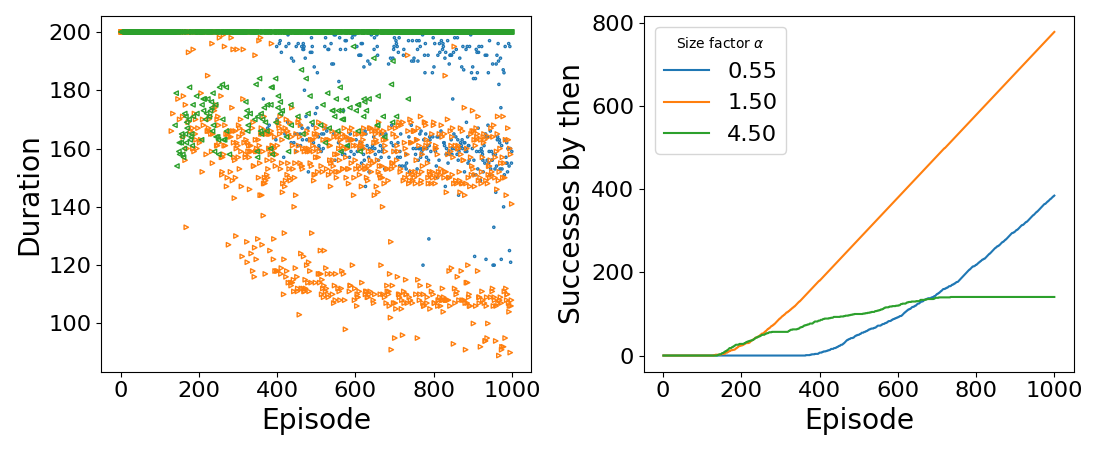
\includegraphics[width=0.67\textwidth]{dyna/dyna_comparison}
            \caption{Duration plots - $N_{eps}$=1000,$k$=3.  }
            \label{dyna-comparison}
        \end{wrapfigure}
        Already for $\alpha=1$, the agent solves the task. 
        To study the performance as a function of $\alpha$, we plot the episode duration evolution and the cumulated number of success in \ref{dyna-comparison} for $\alpha\in\{0.55,1.5,4.5\}$. 
        
        Agents with $\alpha=1.5$ and $\alpha=4.5$ display some successes already before episode 200. $\alpha=1.5$ shows in addition a good performance as the cumulated number of success approaches a line of slope 1 really quickly after that. For this discretization size, a pattern (that will be discussed later) appears. For the lower value $\alpha=0.55$ (fine grained discretization) : the first successes are observed only after around 350 episodes, and the cumulated number of successes approaches a line of slope smaller than 1 (meaning that even after a high number of iterations, some episodes are failures). 
        \begin{figure}[h]
            \centering
            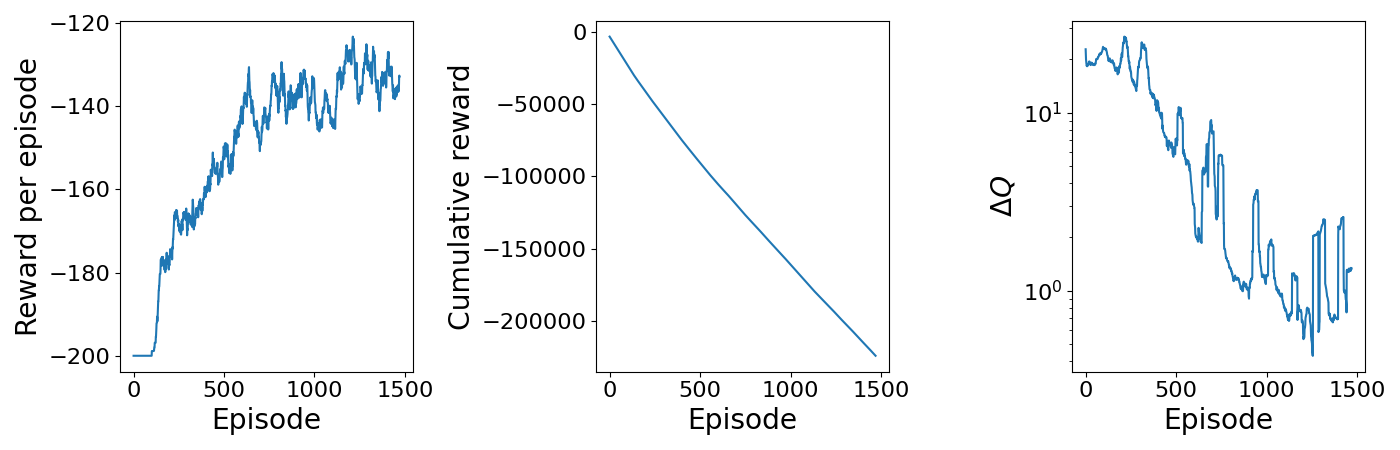
\includegraphics[width=0.9\textwidth]{dyna/dyna-k=3-ss_coef=1.5_eps=8000_final/figs/reward_both_figs_and_deltaQ.png}
            \caption{Reward per episode and cumulated and $Q$-value update - $N_{eps}$=8000, $\alpha$=1.5,$k$=3.}
            \label{fig:reward-both-figs-and-deltaQ}
        \end{figure}

        \begin{wrapfigure}{r}{0.65\textwidth}
            \centering
            %\vspace{-1em}
            \includegraphics[width=0.67\textwidth]{dyna/dyna-k=3-ss_coef=1.5_eps=8000_final/figs/duration.png}
            \caption{Dyna duration plots-$N_{eps}$=8000,$\alpha$=1.5,$k$=3.}
            \label{long-duration}
        \end{wrapfigure}
        $\alpha=4.5$ also shows a poor performance as its number of successes quickly stagnates (less than 150 successes after 1000 episodes). 
        For higher values of $\alpha$, like $\alpha=8$, no success is observed in the first 1000 first episodes. In the same way, for lower values of $\alpha$, like $\alpha=0.3$, the agent completely fails during the 1000 first episodes. Intuitive explanations are given in the very next section.  
        % put the matrix of counts ? saying that it didnt explore much of the space ? 
        \ref{fig:reward-both-figs-and-deltaQ} shows the episode-cumulated rewards and the cumulative rewards (over the episodes) as well as the $Q$-value update step between episodes (defined as the Frobenius distance between $Q$ matrices before and after each episode). That simulation is done with 8000 episodes, using $\alpha=1.5$ and a log-scale $y$-axis is chosen for the $Q$-value update plot.

        Reward per episode starts at -200 and increases quickly to stagnate around -130 on average. Cumulative reward is therefore quasi linearly decreasing. 
        The Q-value update step overall decreases in time. This indicates that the update equation of $Q(s,a)$ converges towards a fixed point. The decrease is however not monotonic. Peaks correspond to reactions of the $Q$-values estimates to new strategy improvements.
        Duration plots in \ref{long-duration} are shown for the same parameters as above but for 10000 episodes. We clearly see a pattern of three blocs of durations appearing. We respectively name them block 1, block 2 and block 3 from top to bottom. Their cause is explained in \ref{sec:characteristic-trajectories}.
        
        \subsection{Why does Dyna work ?}
        Discretizing the state space allows us to map the agent's continuous position and velocity to a finite grid of states, on which the Q-values are initialised at 0. The fact that the episode reward is always $<$0 then promotes exploration. Indeed, the 0 Q-values of the not yet visited states look promising to the algorithm and lead it to try new strategies. This makes it unnecessary to add auxiliary rewards. This in part also explains why fine discretizations lead to slower learning. Indeed, such discretizations increase the amount of state-action pairs that look promising to test out and the number of steps that need to be taken for each Q-value to converge.
        Another contribution for why a slightly coarser discretisation can be advantageous for our environment specifically is that more continuous positions fall into the same discrete state, leading to the assignment of the same action across them. This means the car is encouraged to take repeated actions, which help it build up momentum. On the other hand, if the discretization is too coarse, the agent's behavior is uniform over too large a part of the state space, refraining its adaptation. 
        %Therefore, there is an optimal level of discretization. In our study, we found that this optimal level, where the agent performs best, is around $(\alpha=1.5)$.

        \subsection{$Q$ values table and characteristic trajectories}\label{sec:characteristic-trajectories}
        In the following, we show the estimation of the $Q$ values after learning. In \ref{Qmatrixcounts}, we represent for each state $s$ (located by a position and a velocity) the value $\max_a Q(s,a)$. On top, we represent three trajectories. T$i$ corresponds to a characteristic trajectory from block $i$, $\forall i \in \{1,2,3\}$). Also, the black and red dotted lines respectively correspond to $x=x_0$ and $x=x_r$. 
        The second subplot indicated the set of states that have been visited (1 if visited and 0 if not), while the third shows the number of times each of the states has been visited\footnote{We plot the visited states separately because it was hard to only plot $Q$-values for visited states. We choose to represent the three trajectories in the same plot in order to save space in the report.}. The simulation done for 8000 episodes, $k=3$ and $\alpha=1.5$.
        
        \begin{figure}[h]
            \centering
            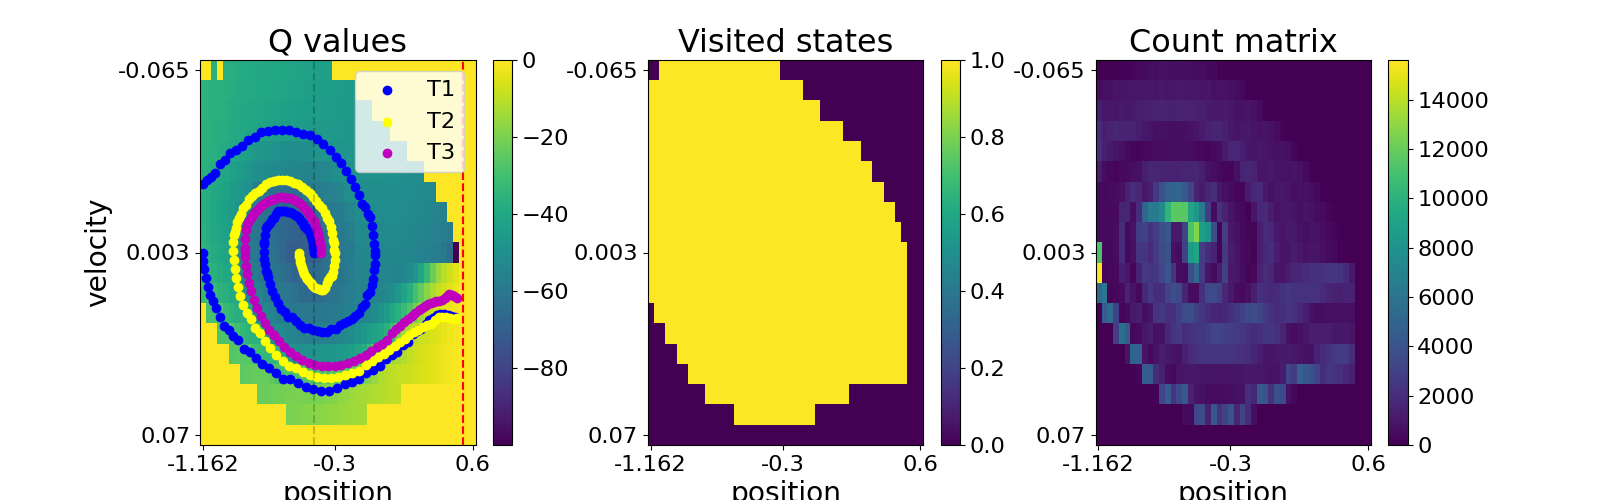
\includegraphics[width=1\textwidth]{dyna/dyna-k=0-ss_coef=1.5_final_Q_and_traj_eps=4000/figs/Q_final_matrix.png}
            \caption{$\max_a Q(s,a)$ table with the three important trajectories, visited states (1 if visited and 0 otherwise), and count matrix - $N_{eps}=4000$, $\alpha$=1.5, $k=3$.}
            \label{Qmatrixcounts}
        \end{figure}

        Interestingly, the $\max_a Q(s,a)$-values shows a spiral starting at the bottom of the mountain and zero velocity. The trajectories follow these spirals. 
        One can notice that in the lower part (positive velocities), when approaching to goal position, $\max_a Q(s,a)$ starts approaching zero. This means that those states are associated to low expected penalization before ending the episode, i.e. they easily lead to the goal.  
        %On the extreme left (and negative velocities), quantity $\max_a Q(s,a)$ has the same value, and this is due to the fact that all those states are "immediate predecessors" of the state on the extreme left position and velocity 0. This is because when the car hits the wall, its velocity immediately drops to zero. 
        By observing the trajectories drawn, we deduce that they correspond to different initial conditions. T3 starts far on the right of $x_0$, allowing it to collect enough momentum to reach the goal with only one swing. T1 starts close to the center, obliging it to swing two times to reach the goal. Notice that it deems advantageous going to the left boundary as fast as possible, even if it means bumping into it and having to again increase its speed from zero. Starting on the left (like T2) leads to taking one swing and a half, whether close or far from $x_0$. 
        The counts matrix illustrates that after 8000 epsiodes, most frequent states are disposed in spirals. A peak of counts is observed for extreme left position and zero velocity, corresponding to cases where the car hits the wall. 
        \section{Comparison of the agents}
        In this section we compare heuristic and RND DQN agents to the Dyna one. We first train the agents for 1500 episodes, and then run each of the trained agents for 1000 additional episodes in `evalutation mode' (i.e. using a greedy policy). Plots of the environment reward evolution during training, as well as evaluation-episodes duration and their KDE are shown in \ref{fig:agent-performance-comparison}. To reduce stochastic fluctuations, the results are made on the same environment seeds across the agents.
        \begin{figure}[h!]
            \centering
            \vspace{0em}
            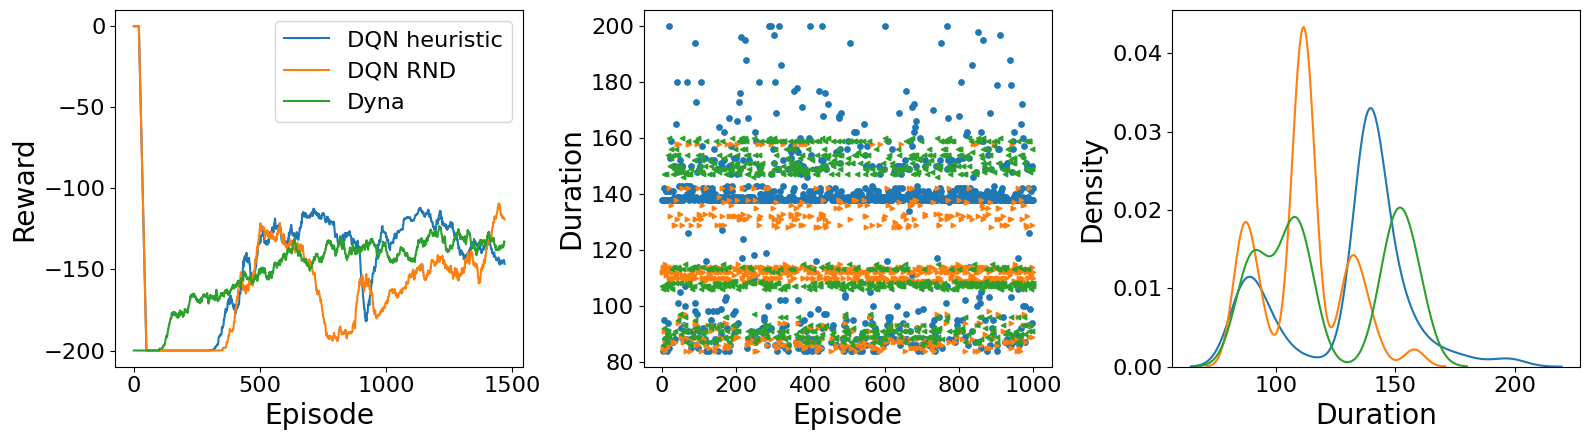
\includegraphics[width=1\textwidth]{../code/comparison}
            \caption{For each agent: environment reward per episode during training, duration plot when testing the trained agents, and KDEs of these durations.}
            \label{fig:agent-performance-comparison}
        \end{figure}
        
        We can see that reward of Dyna is more stable (while others vary more), which suggests it being more reliable than the other algorithms. The KDE plot of durations reveals that the agents find strategies leading to different durations. Overall, DQN-RND seems to have the lowest average duration, making it preferable in term of this metric.  
        \section{Conclusion}
        In this report we analyzed and compared algorithms on the continuous Mountain Car RL environment. We considered versions of a model model-free algorithm (DQN) and a model-based one (Dyna). The algorithm with the best performance was found to be Dyna when valuing learning stability, and DQN with RND auxiliary reward when valuing average success speed (conditioning on a good run). The DQN agent with heuristic reward was found to be the worst performing agent. This can be explained by the fact that it is hard for heuristic rewards not to restrict policy exploration.

        \section{Appendix}
        \subsection{Bonus on Dyna (evolution of $Q$-values)}
        We are selecting three time points: $t_0=100$, $t_1=400$ and $t_2=3600$ episodes to illustrate the evolution of the estimation of the $Q$ values throughout the training. In yellow one can see the states that have not been explored yet (or those for which estimation of the $Q$ value is close to 0).
        \begin{figure}[h]
            \centering
            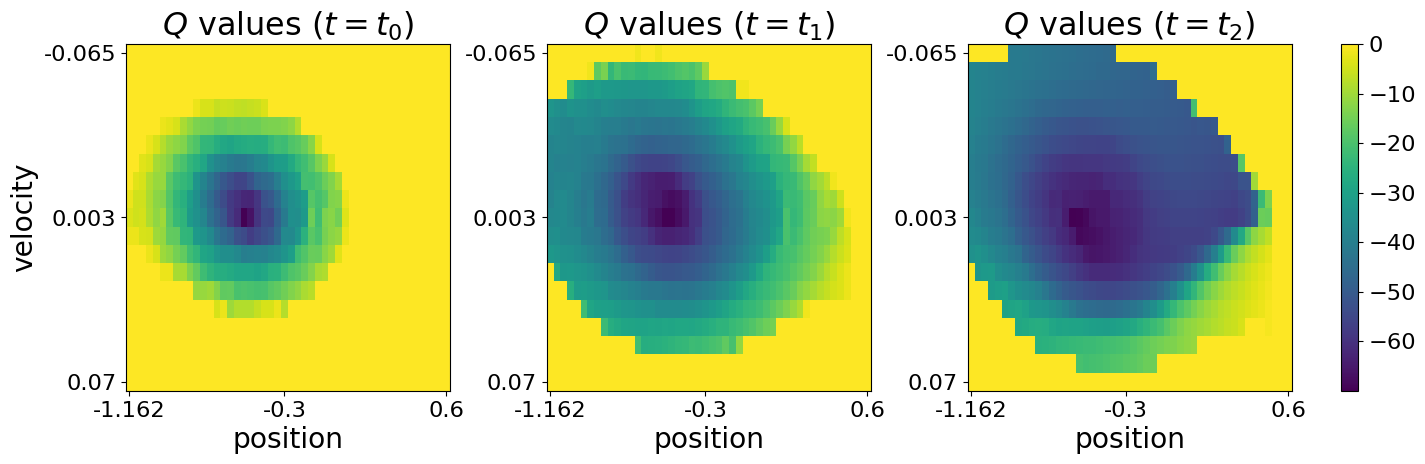
\includegraphics[width=1\textwidth]{dyna/dyna-k=0-ss_coef=1.5_final_Q_and_traj_eps=4000/figs/Evolution_Q_values}
            \caption{$\max_a Q(s,a)$ table at three different times of training $\{t_0=100,t_1=400$ and $t_2=3600\}$ - $N_{eps}=4000$, $\alpha$=1.5, $k=3$.}
            \label{Qmatrixcounts}
        \end{figure}

        We can see that for $t=t_0$, the only $Q$ values that are estimated to be different from zero are the ones in the bottom of the mountain. Indeed, the agent has only explored that region. For a $t=t_1$, the region where the $Q$ values are different from zero gets wider as the agent explores more of the phase space. One can observe a trajectory leading to a terminal state (values that smoothly go from negative values to 0). At that point in time, the agent already shows successes. At a time $t=t_2$, we can clearly observe the spiral structure, and the fact that the spiral widens in the velocity axis. This corresponds to the fact that the agent has learned a quicker way to reach the target (by taking higher velocities in order to get quickly to the destination). We also observe that the agent has learned to reach the goal with a higher final velocity.
        
\end{document}